% Standalone section for the team's existing ICML file.
% Requires graphicx and the bibliography entries in idea5-references.bib.
% Replace provisional discussion after personal review. Do not claim TA approval or human annotation.
\section{Analysis: Availability of Body and Hand Pose in EgoNormia}
\paragraph{Motivation and questions.} Idea 5 proposes adding explicit geometry and body/hand representations to RGB inputs for social-norm reasoning. We examine two premises: whether pretrained extractors produce candidate body/hand representations often enough to supply this pathway, and whether aligned maps provide an immediate benefit to a frozen VLM beyond extra-image and mismatched-map controls. We use EgoNormia's pre-action visual context \citep{rezaei2025egonormia}. This is an output-availability audit and a zero-shot pilot, not a test of pose accuracy or the proposed fine-tuning.
\paragraph{Data and protocol.} We select 40 items from distinct source videos using a fixed SHA256 ordering before detector inference, choosing one item per source. Five frames per pre-action clip are sampled at 10\%, 30\%, 50\%, 70\%, and 90\% of its length (200 frames total). We apply frozen MediaPipe Pose Landmarker Full and Hand Landmarker models in independent-image mode, allowing up to four bodies and four hands. Detection and presence thresholds are 0.5. A body output is retained if at least eight of its 33 landmarks lie within the image and have predicted visibility and presence at least 0.5; we repeat the retention rule at 0.8 as a sensitivity check. The eight-point cutoff is an operational filter, not a validated measure of quality. Hand output means at least one predicted hand; the model does not supply equivalent per-landmark scores. We retain all examples, including blank outputs. Intervals use 5,000 source-video bootstrap samples.
\paragraph{Results.} Body output satisfies the 0.5 retention rule in 59/200 sampled frames (29.5\%) and the 0.8 rule in 59/200 (29.5\%). At least one hand is predicted in 36/200 frames (18.0\%). At least one body or hand output is available in 81/200 frames (40.5\%); 31/40 clips contain such an output in at least one sampled frame. These are detector-output frequencies, not precision, recall, or human-validated extraction quality.
\begin{figure}[t]
\centering
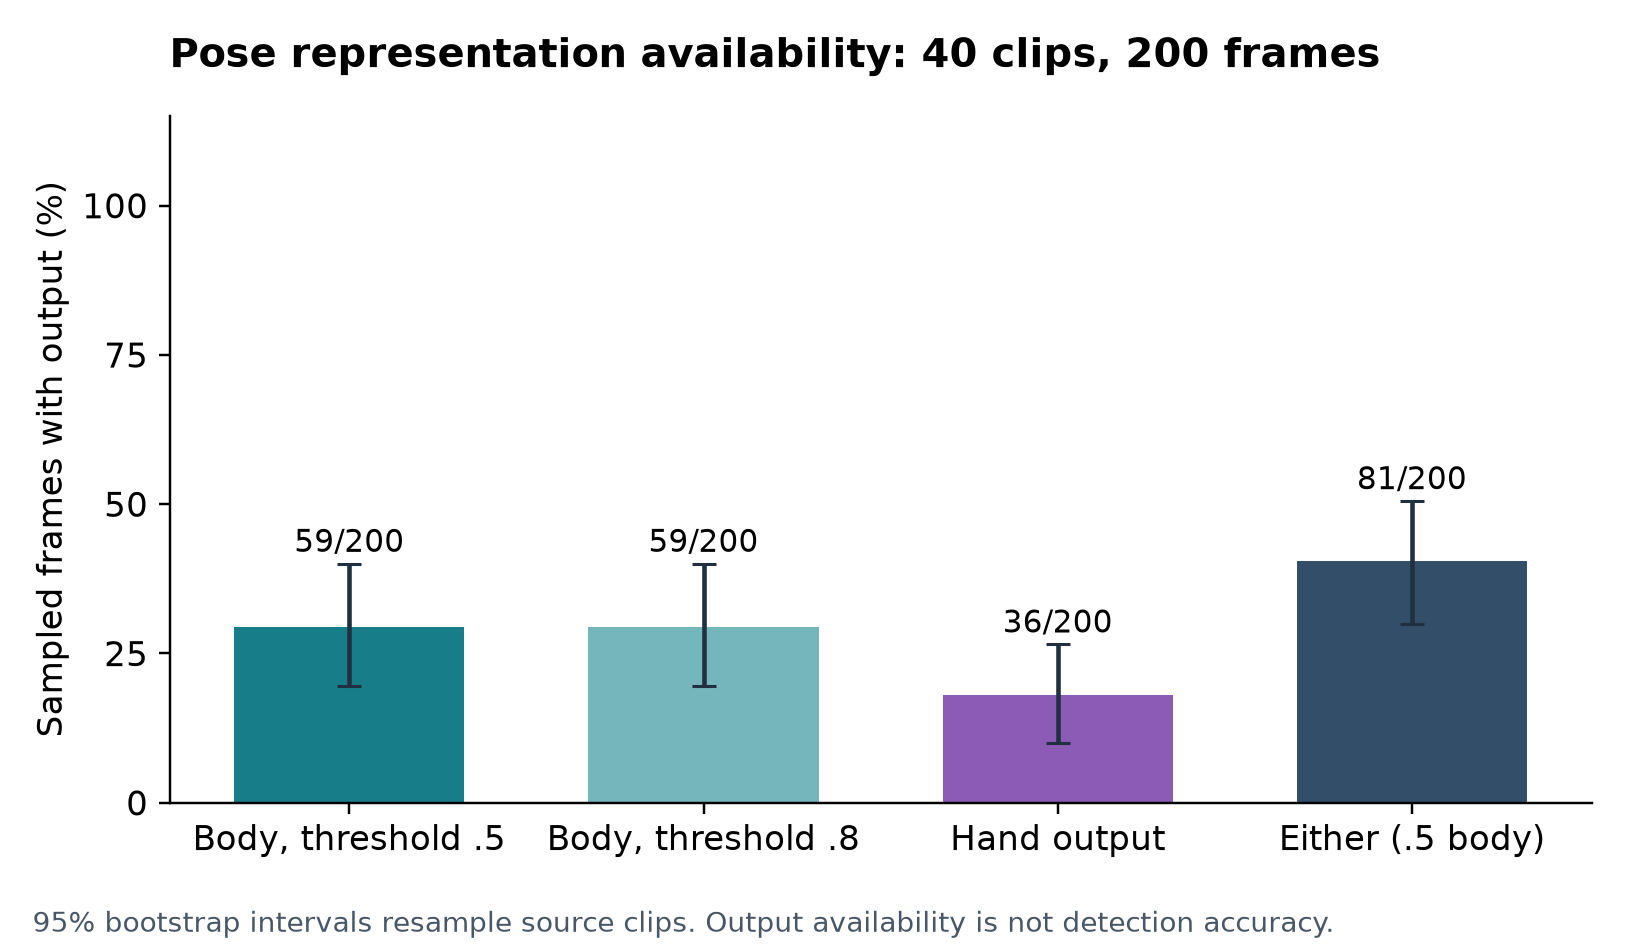
\includegraphics[width=\linewidth]{coverage.png}
\caption{Availability of body and hand outputs on the fixed sample. Error bars are 95\% bootstrap intervals clustered by source video. Body outputs require at least eight retained landmarks; predicted hand outputs use the detector's standard acceptance threshold.}
\end{figure}

\paragraph{Frozen-model pilot.} On the same fixed items, we compare a local community 4-bit Qwen3-VL-8B-Instruct checkpoint under RGB-only, RGB plus repeated RGB, RGB plus aligned body/hand skeletons, and RGB plus skeletons from a different source video. RGB grids contain the same five chronological frames, each resized to a maximum side of 384 pixels; auxiliary grids match target grid dimensions. Repeated RGB controls for the extra image slot, and cyclically shuffled maps test alignment. Greedy decoding separately selects an action and then its justification. Action and justification options are independently permuted per item and kept fixed across conditions; no gold labels, norm labels, or generated descriptions enter prompts. Invalid outputs count as wrong. This is a custom subset pilot, not an official leaderboard replication.
\begin{center}
\small
\setlength{\tabcolsep}{3pt}
\begin{tabular}{lrrr}
Input & Action & Justification & Both \\
\hline
RGB & 18/40 & 19/40 & 16/40 \\
RGB + repeat & 16/40 & 15/40 & 13/40 \\
RGB + aligned pose & 18/40 & 18/40 & 15/40 \\
RGB + shuffled pose & 18/40 & 19/40 & 15/40 \\
\end{tabular}\end{center}
Aligned pose minus RGB joint accuracy is -2.5 percentage points (95\% paired bootstrap interval [-7.5, +0.0]); 0 items improve and 1 worsen. Against repeated RGB, the joint difference is +5.0 points [+0.0, +12.5]. Against shuffled pose, no item's joint correctness changes. The resulting zero-width empirical bootstrap interval is degenerate and does not establish a zero population effect. 

\paragraph{Discussion of this analysis (provisional; author review required).} Aligned pose produces no observed joint-accuracy gain over RGB on this sample, and aligned and shuffled pose have identical joint-correctness outcomes on all 40 items. This provides no evidence of an alignment-dependent benefit under the tested setup. Repeating RGB also changes outcomes, demonstrating why an extra-image control matters. These results do not disprove the fine-tuning proposal: the frozen model has not been adapted to the rendered maps, and the sample is small. Candidate body or hand outputs are available in only 40.5\% of sampled frames; human review must distinguish absent people/hands from detector failures or task-irrelevant detections. Egocentric views can show the wearer's hands without a full body, so both extractors need separate assessment. Five independent frames do not measure motion or identity continuity. Before committing to pose augmentation, manually audit overlays, preserve missing-output indicators, and evaluate adaptation under matched budgets. EgoNormia is excluded from training but has been exposed during exploratory analysis; it should not be described as untouched.

% AUTHOR TASK: Replace the provisional discussion with your observations after reviewing overlays.
% AI DISCLOSURE: An OpenAI Codex agent selected the reproducible sampling rule, wrote and debugged code, downloaded data/models, ran extraction/inference, generated figures and numerical summaries, and drafted this section. MediaPipe generated body/hand landmarks. Qwen generated experimental action/justification predictions. Human review/interpretation is pending and must be attributed truthfully after completion.
